\chapter{Design and Specification}\label{ch_method}

\section{Aim/vision}

The idea of the game is to travel around the world without physically
having to be there, inviting the user to realise the scale of the
world whilst gaining the positive benefits of outdoor exercise. A user
may decide to run around areas in Scotland (the Scotland Mission) and
this is achieved through routes such as Glasgow to Edinburgh. Each
route is further broken up into manageable stages of a few kilometres
and users are awarded badges based on stages/routes completed and
overall distance and time. Therefore the user can gain short-term
success while working towards the satisfaction of larger goals. 

This approach is to examine whether or not this type of encouragement
could potentially work with outdoor exercise. Metrics will be tracked
for individual users to monitor their exercise duration and frequency
and will be used to encourage that user to exercise. These metics will
then be used to form the basis of our conclusion.

The aims of the project are then as follows:

\begin{enumerate}
  \item To provide incentives that become intrinsically
    rewarding. Rewards are primarily linked to stage and route 
    completion and these accumulate to the completion of the entire
    mission - every achievement brings the user closer to a larger
    success. 
  \item To provide long and short term goals to fulfil the sense of
    achievement. The long term goals are Route completion and these are
    fulfilled by the easily achievable short term goals of Stages -
    for example the Central Park Route contains four stages, one for
    each edge of the park and these stages are easily achievable in an
    exercise session.
    \begin{enumerate}
      \item Stage completion - unlock a photograph of the stage or of
        a key landmark near the stage. This is achieved by completing
        a specific stage.
      \item Route Completion - a gold, silver or bronze medal is
        awarded for completing a route in a given time period. A route
        is completed when all the stages in a route are completed.
    \end{enumerate}
\end{enumerate}


\section{Specification}
\label{sec:specification}
The implementation specifics of this project are defined herein with
the overall development of the project shown in the following sections.

An overarching goal for this implementation is to minimise the end cost
for the user. This cost takes two forms: response time for data
loading and network costs incurred through data loading.

Initial response time for loading data cannot be avoided without
prepackaging content inside the app. We do not want the user to be
forced to update the app every time we want to add another route to
run down so prepackaging will not work. We can however cache the data
we know does not change and reference that instead - which is much
faster than a network response time.

Caching also reduces the overall network cost: by caching the data
received we remove the need to make the request again. This inherently
reduces the network cost by reducing the number of network requests.

These are discussed in more detail in Section \ref{sec:notable} and
will be referenced in the following subsections.

\subsection{Platform and Frameworks}
The mobile application is developed using PhoneGap \cite{phonegap}, 
a tool which allows you to develop a mobile app as if it were
a web app, and then package it as a mobile app. The decision to use
PhoneGap instead of building a native app is primarily because I come
from a web development background but also so we can deploy to
multiple platforms easily without needing to change the code base. 

Because of this, our application is written using HTML, JavaScript,
and CSS3. The twitter Bootstrap CSS framework \cite{bootstrap} was
used because of the excellent support for small screen devices and
layout management. 

Titanium, developed by appcelerator\cite{titanium}, is an alternative
platform to PhoneGap that was also considered. This required a greater
knowledge of android than PhoneGap does but the biggest drawback was
the state of development when the project started. After discussion
with members of the startup community who were using Titanium, it was
apparent that Titanium was still a work in progress and probably a
risk to go with. The platform is now flourishing and would probably
have been the better choice to go with in retrospect, but at the
begining of the project the safer choice was to develop for PhoneGap.

AngularJS\cite{angularjs} is the framework used for the
application. This framework has a major benefit of explicit data linking
between the DOM(Document-Object Model) and the javascript controlling
that section of the DOM. In AngularJS, a controller is defined to
manage the behaviour of a specific section of a page. By defining
these controllers, we can utilise this explicit data linking to manage
how information is displayed in the DOM - if a variable changes in a
controller then it also updates in the DOM. This linking is
bi-directional, so the reverse is also true. 

The AngularJS framework also facilitates many other control
mechanisms: DOM tree manipulations, CSS class manipulations, frontend
routing (a process where a section of the DOM tree and an associated
JavaScript controller are swapped out based on the current URL) and
wrappers around the browsers native AJAX implementation. All of this
functionality make AngularJS the ideal framework for the project. 

The web application is written in Python and uses Django\cite{django}
and Django-Tastypie\cite{tastypie}. Django is used as a middleware
platform for interfacing with the database and creation of specific
workflow interactions; while Django-Tastypie is used for managing and
building a REST style API for well-defined database object access.

Django exposes an Object-Relation Mapping (ORM) inside the framework
for manipulating and creating database objects. This is utilised by
Django-Tastpie for creation of the REST API. We use a REST style API
so that the mobile app is able to uniquely identify an object in the
database in a consistent and reliable manner. This is used in 
session management in Section \ref{sec:session_mgmt}.

Moreover, there is a large number of database objects that we require
knowledge about in the app. A tool which creates a well defined way of
accessing these objects and managing their access permissions is
invaluable for consistency and reliability.

No session-like state is required in this application as the database
object relations are defined in such a way that they hold all
information required. 

\subsection{N-Tier Diagram}
The high level components of this system are reasonably simple (figure
\ref{NTier}). The
user requires a mobile phone with GPS enabled, an active internet
connection and the mobile application installed. This communicates
with a Django Webserver with a REST-style API (with a small number of
bespoke views since some behaviour does not fit well with the REST
specification) which in turn uses Django's Object Relation Model (ORM)
to persist these to a database.

The mobile application communicates with the devices GPS location
management system to obtain location information for the
user. We request that the users devices provides us with the most
accurate GPS location it can provide, so it will try satellite
positioning first and then try network provided information.
\begin{figure}[H]
  \centering
  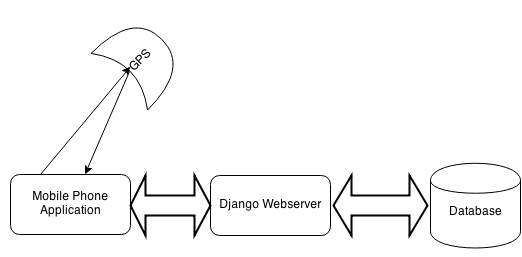
\includegraphics[width=\textwidth]{images/N-tier.png}
  \caption{N-Tier diagram}
  \label{NTier}
\end{figure}

\subsection{Entity Relation Diagram}
\label{sec:ER}
There have been two significant iterations of the Entity Relation (ER)
diagram in this project - the first (figure \ref{ER_1}) is the final
theoretical ER model and the second is the real world implementation
with modifications and extra linking for data transfer optimisation
and changing requirements.

The main reason for the implementation modifications is to keep data
transfer low between the mobile device and the API. Since the mobile
device will be using non-wifi based communication methods the number
of bytes transferred will be logged by their network provider and will
cost the end user. Since we care for the monetary cost that using the
app may incur to the end user (Section \ref{sec:consideration}), we can
sacrifice having a non-redundant database in order to optimise the
data transfer for the end user.

\begin{figure}[H]
  \centering
  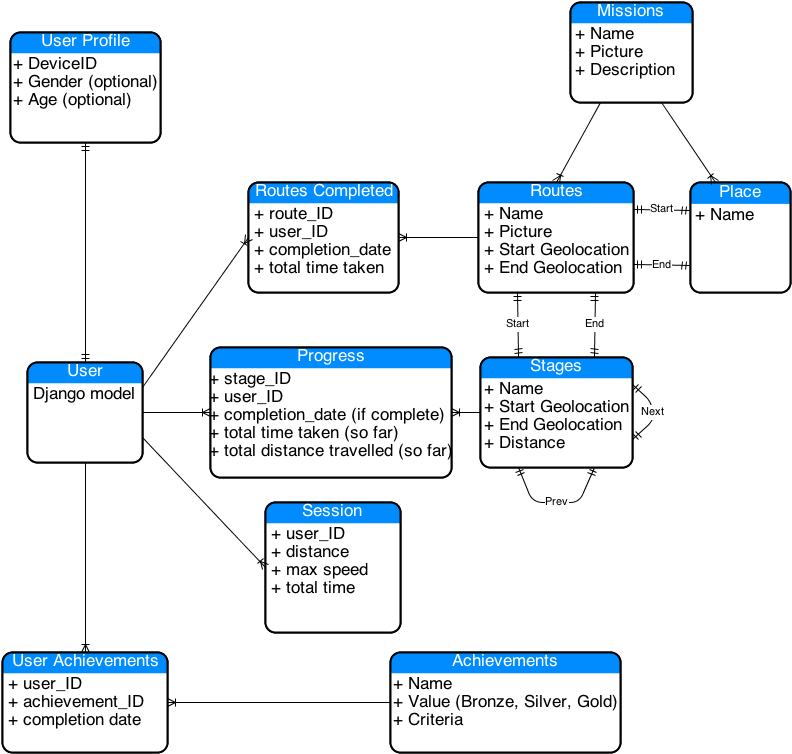
\includegraphics[width=\textwidth]{images/ER.png}
  \caption{ER diagram, final theoretical model}
  \label{ER_1}
\end{figure}

\todo{Do implementation ER diagram}



\subsection{Walkthrough of Wireframes}
\todo{THIS NEEDS REDONE WITH NEW WIREFRAMES}

When the app is launched it silently registers with the server
allowing the user to use the app immediately. The user is then shown
the middle-top screen.
\begin{enumerate}
\item From the middle top screen, the user can follow arrow 1 by
  clicking on the middle button ``Pick Mission'' to pick a Mission
  (Run around Arran or Egg for example) and then pick a start and
  end location. After confirming these choices, the user is taken
  back to the middle top screen, or at any time can click the
  ``Home'' button to return. 
\item The user can also view their current acheivements by clicking
  the ``Achievements'' button on the middle top screen, following
  arrow 2. These achievements will be grouped by tabs by category -
  Distance, Time, Stage and Mission based achievements.
\item The user can follow arrow 3 from the middle top screen to
  notify the app that they are starting an exercise period, telling
  the app to track their distance. If a Mission and start and end
  location are not picked (as in point 1) then they will instead be
  redirected to this screen and are unable to start exercising until
  this choice has been made. Once they have successfully advanced to
  this screen, it will display their current progress as they move
  showing the user how close to completion of their current stage
  and overall route they are. 
\item When the user has finished exercising, they will click the
  ``End Session'' button and be taken to the first summary screen -
  following arrow 4. Here statistics from their exercise will be
  shown and the option to share this on several social media
  outlets.
\item The user can then move to the second and final summary screen,
  following arrow 5, where they will be shown any achievements they
  were awarded during that session. The user will also have the
  option to share these on social media outlets. From here, the user
  can click the ``Home'' button and be taken back to the middle top
  screen. 
\end{enumerate}
\begin{figure}[H]
  \centering
  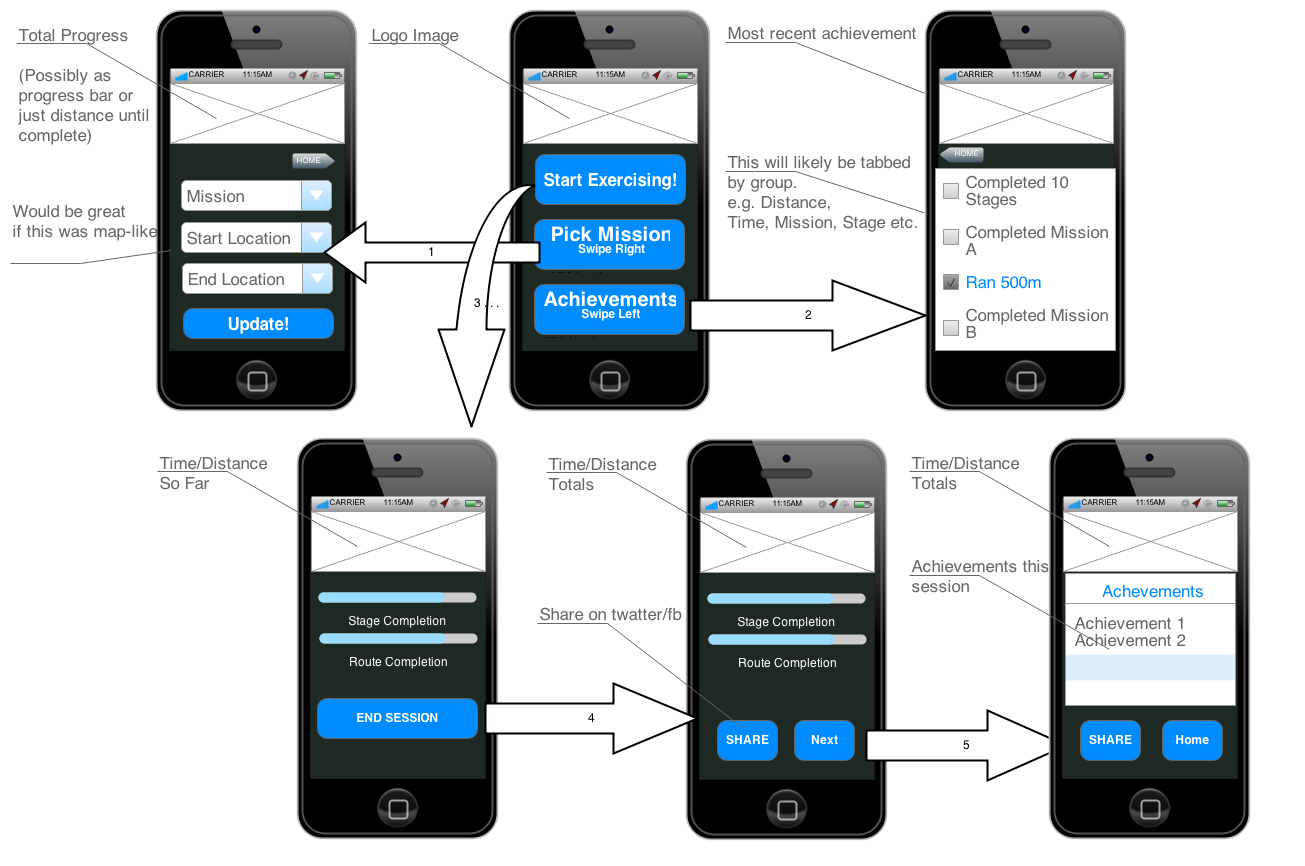
\includegraphics[width=\linewidth]{images/Wireframes.png}
  \caption{Wireframes, initial design}
  \label{wireframes_1}
\end{figure}

\section{Notable design decisions}\label{sec:notable}
\subsection{Explicit caching}
\label{sec:explicit_caching}
As was mentioned in Section \ref{sec:specification}, the minimisation of network
traffic is of great consideration when dealing with mobile devices. We
did not want the mobile device to make repeated API calls for
resources that will not change in the short term - resources such as
what missions are available, what routes belong to what missions and
what stages belong to each route. 

The main case for this is as follows. A user may open the app for the
sole purpose of browsing all missions and their routes, and any
progress they have on these routes before they start using the app for
exercise. In an unmanaged situation the app could call the API each
time it lands on a menu to pick a mission or the routes for a mission
- if the user is browsing then they may see the same information
provided several times. 

If we remove data transfer from the equation all together and focus
solely on the user experience then caching will give a better user
experience in terms of loading speed. Since caching means we do not
have to hit the API each time we want to see something we have seen
before, we can load selection menus faster. 

Note that only data endpoints that are unlikely to change in the short
term or those that cannot feasibly change under certain circumstances
are cached. The ``progress'' endpoint which provides the data about a
users progress along given stages will not change if the user does not
initiate an exercise session - the user has not made any more progress
so it could not have changed.

These caching services are used as singleton-like facilities in the
application to ensure consistent data throughout the application, an
update to this data will be reflected throughout the entire
application. 

\subsection{Promise Based Module Interfaces}
Each module that has been created for managing either a specific set
of objects(routes, missions or the user object) has been defined
with a common interface. This common interface brings a regular
and well defined way of interacting with these modules, especially if
they utilise explicit caching (section \ref{sec:explicit_caching}) or
execute asynchronous methods.

There are two ways that this consistent interface could be
implemented: a function callback explicitly provided as an argument to
the module function call; or by using promises.

Function callbacks passed as parameters are a common JavaScript
paradigm. They are used in the PhoneGap framework to interface with
the device\cite{phonegap_currentpos}. A frequent problem with function
callbacks is what is colloquially known as ``callback hell''
\cite{callback_hell} where nested anonymous functions are used to
bring an order of execution to asynchronous tasks. This can become
unmanageable and hard to maintain in larger projects but can be
overcome with good software development procedures. An example of how
the callback approach works is show in Figure \ref{fig:callbacks}.

\begin{figure}[h]
\begin{verbatim}
function async(callback){
  // Do something with the args asynchronously.
  // Then explicitly call the callback function.
  callback(data);
}

function callback(data){
  // do something with the data returned from the asynchronous task.
  console.log(data);
}

// Invoke the asynchronous function and process the returned data.
async(callback);
\end{verbatim}
\caption{Callback approach to asynchronicity}
\label{fig:callbacks}
\end{figure}

The biggest problem for us is the framework we are using - AngularJS
only knows about events that happen in its own scope. This means that
when we invoke the callback function with the data from a module, the
data will be updated in the controller but AngularJS does not know to
update any reflections of this data in the DOM or elsewhere. There are
ways to notify the framework that it should run an update (known as a
digest cycle)\cite{angularjs_apply} but if we invoke this when a
digest cycle is currently in progress then the framework throws an
error and drops the request.

Another option is to use the AngularJS wrapping for the standard
``setTimeout'' function with a delay of zero. The ``setTimeout''
function executes a callback function after a certain time
period\cite{setTimeout}. While this may seem
frivolous, a subtlety of this wrapping avoids the digest cycle clash
of the above problem. The AngularJS wrapper ``\$timeout'' will invoke
the function passed to it after the delay expires, but importantly
will cause a natural digest cycle to occur. So if this is called using
a delay of zero then we make AngularJS update without risk of the
framework erroring. This is the method that we use inside the ``core''
set of modules that wrap the PhoneGap device API
methods\cite{wrappingPhonegap} as they use callbacks as their own
notification method. Wrapping using ``\$timeout'' can be shown in
figure \ref{fig:timeout} (note this is an example that is stripped of
the necessary declarations to work in the framework, it is intended as
an example only).

\begin{figure}[h]
\begin{verbatim}
\\ PhoneGap function to get the users location,
\\ success and failure are two callback functions.
\\ Note the similarity to the previous example.
geolocation.getCurrentPosition(callback)

\\ This is defined in our controller or other module.
function success(data){
  \\ Call the $timeout function with delay of zero to safely invoke
  \\ on next digest.
  $timeout(function(){
    \\ do something with the location data
    \\ AngularJS knows about this update.
  }, 0);
}

\\ Invoke request for location information.
geolocation.getCurrentPosition(success);
\end{verbatim}
\caption{Using ``\$timeout'' to wrap PhoneGap API}
\label{fig:timeout}
\end{figure}

Internally within modules the ``\$timeout'' method is used for
notifying the framework of necessary change as PhoneGap uses callbacks
as its own notification method. Callbacks could also be used for
inter-module communication but would require each callback function to
use the ``\$timeout'' method if any asynchronicity occurs. Since we
want to develop a consistent interface between all modules this is not
appropriate: we need to know when we should and should not require a
call to ``\$timeout'' when we write the callback function, and this
can be different between modules.

We can remove all these complexities by using promises. A promise
allows us to manage deferred (asynchronous) callbacks and synchronous
callbacks in the same way and the AngularJS framework has promises
integrated in with the digest cycle management. 

Promises and callbacks are theoretically similar as both provide a
function to be called once something has occurred however promises do
not suffer from the ``callback hell'' anti-pattern that callbacks
alone do due to a flow control change.
Kris Kowal, the creater of the promise library ``Q'' that
AngularJS bases its promise library ``\$q'' on, defines the flow
control change as follows:
\begin{quote}
The callback approach is called an ``inversion of control''. A function
that accepts a callback instead of a return value is saying, ``Don’t
call me, I’ll call you.''. Promises un-invert the inversion, cleanly
separating the input arguments from control flow arguments.\cite{kriskowalq}
\end{quote}

A function that uses promises to notify success or failure immediately
returns a promise object. This is different to the callback approach
as the program is allowed to continue to execute as the function
immediately returns, unlike the callback approach which blocks for the
response, and the function to handle the response is invoked when a
response is ready. These response handlers are attached to the promise
object by calling the ``then'' method of the promise, and these are
called when the promise resolves. This can be shown in Figure
\ref{fig:promises}. 

\begin{figure}[h]
\begin{verbatim}
// This could be in another module, but doesn't need to be.
function promiseFn(){
  \\ Create a new promise
  var deferred = $q.defer();
  var data = {}; \\ Data from (a)synchronous task stored in here.  

  \\ Something asynchronous or sychonous here. Once it's completed...
  \\ Resolve the promise
  deferred.resolve(data);

  \\ return the promise
  return deferred.promise;
}

function processData(data){ ... //Do something with data }

// Call function and process the data it returns.
promiseFn()
  .then(processData);
\end{verbatim}
\caption{Using Promises in AngularJS}
\label{fig:promises}
\end{figure}

Although promises are intended for use when there is asynchronous
behaviour, they can also be used in synchronous situations. The exact
user-perceived behaviour would also occur if the asynchronous task was
made synchronous in figure \ref{fig:promises}. The functions passed to
the ``then'' method of a promise will be called when the promise is in
a state of being resolved, so they can be added before or after the
promise is resolved and they will be called in both cases.

This then provides us a method that allows a consistent interface that
integrates well with AngularJS. It is worth noting that the
``\$timeout'' method is used with modules that interface with any of
the PhoneGap device API methods that are asynchronous. As is discussed
previously, this is to notify AngularJS that a promise has changed
state in a situation that it does not know about. So although promises
solve most of our problems, they do not completely solve all of them.

\subsection{Exercise Session Management}
\label{sec:session_mgmt}
Due to the environmental implications brought on by GPS, we may not be
able to identify their location. The user should not
be penalised for this as it is outwith their control and is not a
direct error on their part. Something as simple as running through a
tunnel could initiate the loss of signal. 

To counter this, the exercise session is designed in such a way as to
not penalise or disadvantage the user if they should not be able to
obtain location information. 

When a user decides to exercise, a new session is created through the
API. The users device is then given a unique ID for that session that
only they have a knowledge of (in the first iteration of this
implementation this ID is a direct mapping to the ID of the object in
the database, but in a future version this could be something more
obscure). Only this user can update this session and it can only be
updated if you know the unique ID for that session. 

This ID is saved on the users device for the duration that the user
wants the session to be active and is deleted when the user either
closes the app or explicitly ends the session. We can then update the
session sucessfully when we have a GPS location and are ready to
update, while indirectly ``ending'' the session when we delete the
unique ID.

If the user cannot obtain location information then the device will
retain the unique ID for the session and will update as soon as it can
obtain location information. This is explored further in section
\ref{sec:location_mgmt}.

This does guarantee that the user will gain all distance they should
be awared. If the user starts an exercise session but cannot then
obtain location information and either exits the app or ends the
exercise session then the user will not be credited for the distance
they travel. This is a situation we cannot control and so we can
accept that this is a limitation of the implementation.

When a session is created we need to tell the server what route we
intend to travel down and where we currently are (in terms of our
longitude and latitude). To update a session, we only need to provide
a timestamp, longitude and latitude positioning and the session
ID. On receipt of a successful update the server will update what
stage a user is on, automatically moving the user onto the next stage
on a route when they complete their current stage. 

Only the last known location (set of longitude and latitude
coordinates) and the time that the user was at those coordinates are
kept in the server. We only need the last location 
to work out distance a user has travelled since the last update. 

We have two options when a user completes a stage: we can either
accumulate the excess distance they travel and allow the user to
``spend'' this distance on whatever route they like when they finish;
or automatically advance the user onto the next sensible route. 

The latter option was chosen for this implementation as it is the most
immersive option of the two. From a game perspective, the first option
does not allow the user to fully engage in the game at the time they
are playing as no further rewards are accumulated when distance is not
being incremented while the second allows the user to continue
progressing seamlessly. 

\subsection{Location Management}
\label{sec:location_mgmt}
Phonegap exposes two main ways to obtain location information, either
by requesting where the device is at this exact moment in
time\cite{phonegap_currentpos} or by requesting to be updated at a
discreet time interval when the device position
updates\cite{phonegap_watchpos}. 

The original intention was to use the first method to manually control
the time between requesting new location information so that if a
request fails we can immediately send a request again. This method was
dropped after closer inspection of the plugin that provides these
services and research into how the Android Location Manager handles
location data.

The plugin that provides the location data links directly to the
Android Location Manager as expected. This location manager handles
all requests for location data from all applications running on the
device. The second method of obtaining location information registers
a watcher with this Location Manager and allows the Location Manager
to handle the polling for coordinates. If location information cannot
be obtained then we rely on the Location Manager to deal with
retrying. 

As much as we may wish to immediately retry searching for coordinates
with the intention of keeping accurate distance information for a
user, this may have negative repercussions. Obtaining accurate
location information is a costly operation requiring 50mA for each set
of coordinates, more when there is no recent location
information\cite{android_power}. It is the fourth most power intensive
operation an app developer can invoke, as shown in figure
\ref{fig:power} \cite{android_efficiencySlides}.

\begin{figure}[h]
  \centering
  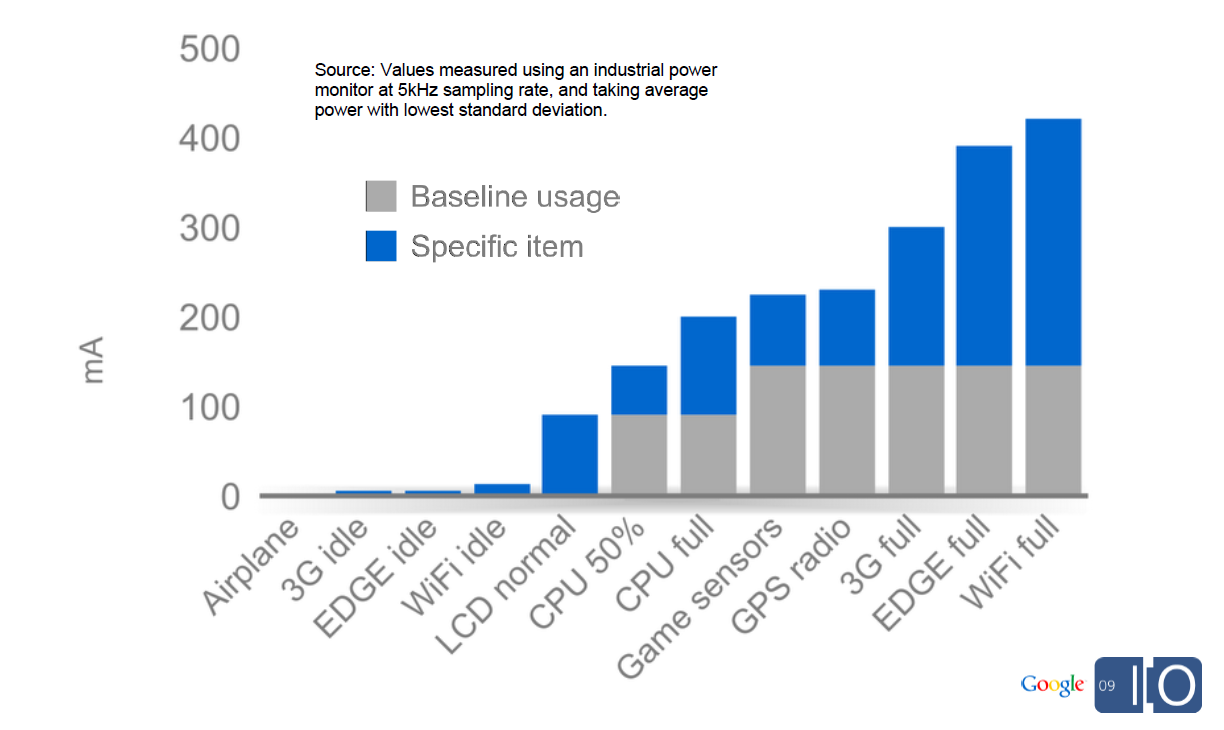
\includegraphics[width=\textwidth]{images/power.png}
  \caption{Power Consumption of sensors on Android Devices \cite{android_efficiencySlides}}
  \label{fig:power}
\end{figure}

In the situation where we will not be able to obtain location
information, when a user enters a tunnel for example, it would be
unnecessary to repeatedly ask for location information. The only
outcome in this scenario is a faster drain on the users battery which
could lead users to have a negative experience with the app. So even
though we are leading with the best of intentions it is not the right
decision to make. Due to the round trip time required to notify the
server of new location information and the relatively short distances
users can travel, it was decided that the provided interval of one
update a minute was sufficient to ensure a balance between power and
accuracy. 

Polling for location information once a minute does suffer from one
drawback we will define as the ``Cul-de-sac Effect''. The Cul-de-sac
Effect arises between two location updates where the user travels a
significant distance between these two updates but these location
updates occur close to one another, resulting in a much smaller
perceived distance. This effect arises when we reduce update
frequency to increase power conservation and can be shown in figure 
\ref{fig:cul-de-sac} where we assume all location updates (noted as
``GPS Location'') occur consistently at a discreet time interval. 

\begin{figure}[h]
  \centering
  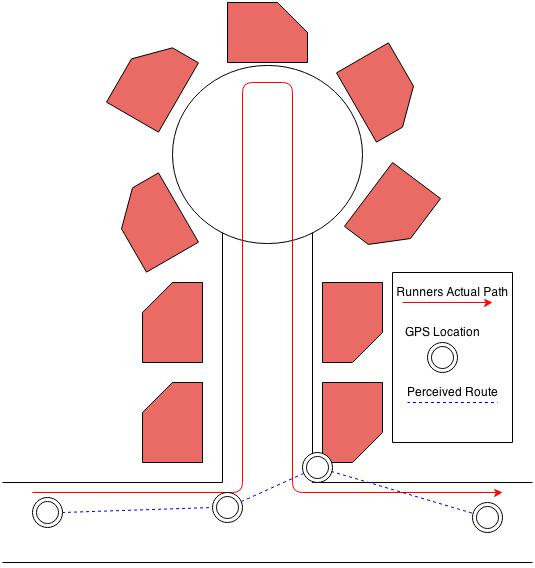
\includegraphics[width=0.7\textwidth]{images/cul-de-sac.jpg}
  \caption{Example of the ``Cul-de-sac Effect''}
  \label{fig:cul-de-sac}
\end{figure}

In the contrived example shown in figure \ref{fig:cul-de-sac} we have
no evidence that the user has travelled into the cul-de-sac, as we
base our distance calculations solely from the location information,
and so we cannot award them the distance they have actually
travelled. Therefore the user is unnecessarily penalised through the
unfortunate circumstances of timing and their route choice. 

As is noted in Section \ref{sec:distance_ver}, the maximum speed we
allow users to travel at is $\text{6}m/s$. In the worst case of this
effect the users device will return location information that informs
us the user has moved no distance (the coordinates are exactly the
same). If we assume that we receive the location updates exactly once
a minute then the worst case distance that the user could lose due to
this effect is $\text{360}m$ . This is a considerable distance and the
unacknowledged effort could have a large negative effect on the
user. Futher work is required to analyse this effect to find the best
update frequency interval with respect to this effect and power
consumption. 


\subsection{Distance Verification}
\label{sec:distance_ver}
To create an exercise session a set of longitude and latitude
coordinates are required. By enforcing this requirement we are always
able to know where a user was last and then work out the distance they
have travelled when new coordinates are provided. 

Converting two pairs of longitude and latitude coordinates to a
distance in kilometers is done through the Haversine
Function\cite{haversine} with a python module of the same
name\cite{python_haversine}.

We send the coordinates to the server and compute the distance there
instead of on the mobile device in the interests of verifying that
the distance is correct. If a user only sends a distance and not a
set of coordinates then we have no mechanism of determining if that
distance is valid or not, whereas if we are given coordinates then we
have a reference point to compare to (since we retain the last known
coordinates). It can be argued that even this is not enough to fully
guarantee that the location information provided is honest but there
is little we can do to ensure honesty in this case. 

We can however limit the distance we update by based upon whether or
not that distance is physically possible. A timestamp is required when
updating with a set of coordinates and so we can compute the speed the
user was travelling at over the time period since their last
update. If this speed is greater than a fixed maximum travel speed
then action is taken to reduce the distance to the maximum distance
the user could have travelled in this interval. This process is shown
in Figure \ref{fig:distance_limit}.

\begin{figure}[h]
\begin{equation}
  distance = haversine(coordinates_{old}, coordinates_{new})
\end{equation}
\begin{equation}
  time = timestamp_{new} - timestamp_{old}
\end{equation}
\begin{equation}
  speed_{actual} = \frac{distance}{time}
\end{equation}
\begin{equation}
  distance = \left\{
  \begin{array}{l l}
    distance & \text{if $speed_{actual} \leq speed_{max}$} \\
    speed_{max} \times time & \text{if $speed_{actual} > speed_{max} $}
  \end{array}
  \right\}
\end{equation}
\caption{Limiting the distance a user can travel based on a maximum speed.}
\label{fig:distance_limit}
\end{figure}

The maximum speed we allow users to travel at is $\text{6}m/s$ as this
accommodates for sprinting and will facilitate cyclists, should they
wish to use this app.

This action to limit the distance travelled based on the time period
will help to defend against cheating but will not negatively impact
users who cannot obtain location information for an arbitrary time
period. A user could still upload bogus coordinates to the server but
this limiting will help to reduce the effectiveness of their
cheating.



